\chapter{Ajuste de controlador difuso basado en descenso del gradiente}
\label{ch:fuzzy-controller-adjustment}


Como vimos en la sección~\ref{ss:fcs} del capítulo~\nameref{ch:sota-ci}, un \ac{fcs} se compone de cuatro bloques diferenciados: la fuzzificación, el bloque de reglas, la inferencia y la defuzzificación. De éstos bloques, el proceso manual de ajuste se resume siempre\sidenote{
	Por supuesto implica más ajustes como la elección de las funciones de fuzzificación, las $t$-normas y $t$-conormas, de la función de defuzzificación, pero estas operaciones no tienen tanto impacto en el desempeño del controlador como las particiones difusas y las reglas.
} en dos pasos:

\begin{enumerate}
	\item Elección de las particiones difusas de las variables lingüísticas.
	\item Definición de las reglas difusas.
\end{enumerate}

Las soluciones de ajuste que existen en la literatura suelen funcionar ajustando automáticamente uno de los dos puntos manteniendo constante el otro (e.g. ajustar las particiones manteniendo fijas las reglas). Nosotros representaremos el controlador como un grafo computacional de manera que sus gradientes sean sencillos de ajustar\sidenote{
	Como veremos más adelante, el tiempo de ajuste con esta representación es muy rápido, lo que abre la posibilidad de desarrollar un algoritmo que incluya este para el ajuste de los metaparámetrosdel controlador, como por ejemplo los tamaños de las particiones.
}.

\newthought{El bloque de fuzzificación} está compuesto por variables lingüísticas, compuestas por conjuntos difusos definidos por funciones de pertenencia. Estas funciones de pertenencia son las que definen las particiones y son las que contienen los parámetros ajustables. Nosotros usaremos la línea ascendente, la línea descendente y el trapecio.

\begin{marginfigure}
	\missingfigure[figwidth=\textwidth]{Line desc}
	\caption{Función de pertenencia linea descendente definida por $(a, \delta b)$.}
	\label{fig:line-asc}
\end{marginfigure}

\begin{marginfigure}
	\missingfigure[figwidth=\textwidth]{Line asc}
	\caption{Función de pertenencia linea descendente definida por $(a, \delta b)$.}
	\label{fig:line-desc}
\end{marginfigure}

\begin{marginfigure}
	\missingfigure[figwidth=\textwidth]{Trapz}
	\caption{Función de pertenencia linea descendente definida por $(a, \delta b, \delta c, \delta d)$.}
	\label{fig:trapz}
\end{marginfigure}

\begin{figure}
	\centering
	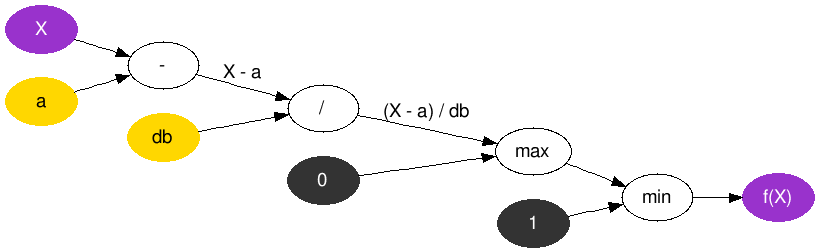
\includegraphics{slope-asc-graph}
	\caption[Grafo computacional de la función de pertenencia para la línea ascendente]{Ilustración del grafo computacional para la función de pertenencia línea ascendente. La fórmula que describe es $\mu(x) = \min(\max(\frac{x - a}{\delta b}, 0), 1)$, quedando acotada $\mu(x)$ en el intervalo $[0, 1] \in \mathbb{R}$. El grafo computacional para la línea descendente es similar y se corresponde con la fórmula $\mu(x) = \min(\max(\frac{a - x}{\delta b + 1}, 0), 1)$.}
	\label{fig:slope-asc-grap}
\end{figure}

Las líneas \textbf{ascendente} y \textbf{descendente} tienen una forma parecida. El grafo asociado a la fórmula de la línea descendente se muestra en la figura~\ref{fig:slope-asc-grap}, que es la que se correspondería con el último conjunto de una partición difusa. Como se puede ver, las variables ajustables son $a$ y $\delta a$. Estas definen el intervalo $(a, a + \delta b) \in \mathbb{R}$ donde los valores $f(X)$ ascienden de $0$ a $1$ (o descienden de $1$ a $0$ en el caso de la recta ascendente).

El \textbf{trapecio} se define a partir de los parámetros $(a, \delta b, \delta c, \delta d) \in \mathbb{R}$, que definen los intervalos $I_1 = (a, a + \delta b)$, $I_1 = (a + \delta b, a + \delta b + \delta c)$ y $I_3 = (a + \delta b + \delta c, a + \delta b + \delta c + \delta d)$. $I_1$ es el intervalo donde la función de pertenencia aumenta su valor de $0$ a $1$, $I_2$ el intervalo superior del trapecio donde la función vale $1$ e $I_3$ donde la función comienza a descender su valor de $1$ a $0$. El grafo asociado a esta función se ilustra en la figura~\ref{fig:trap-graph}

\begin{figure}
	\centering
	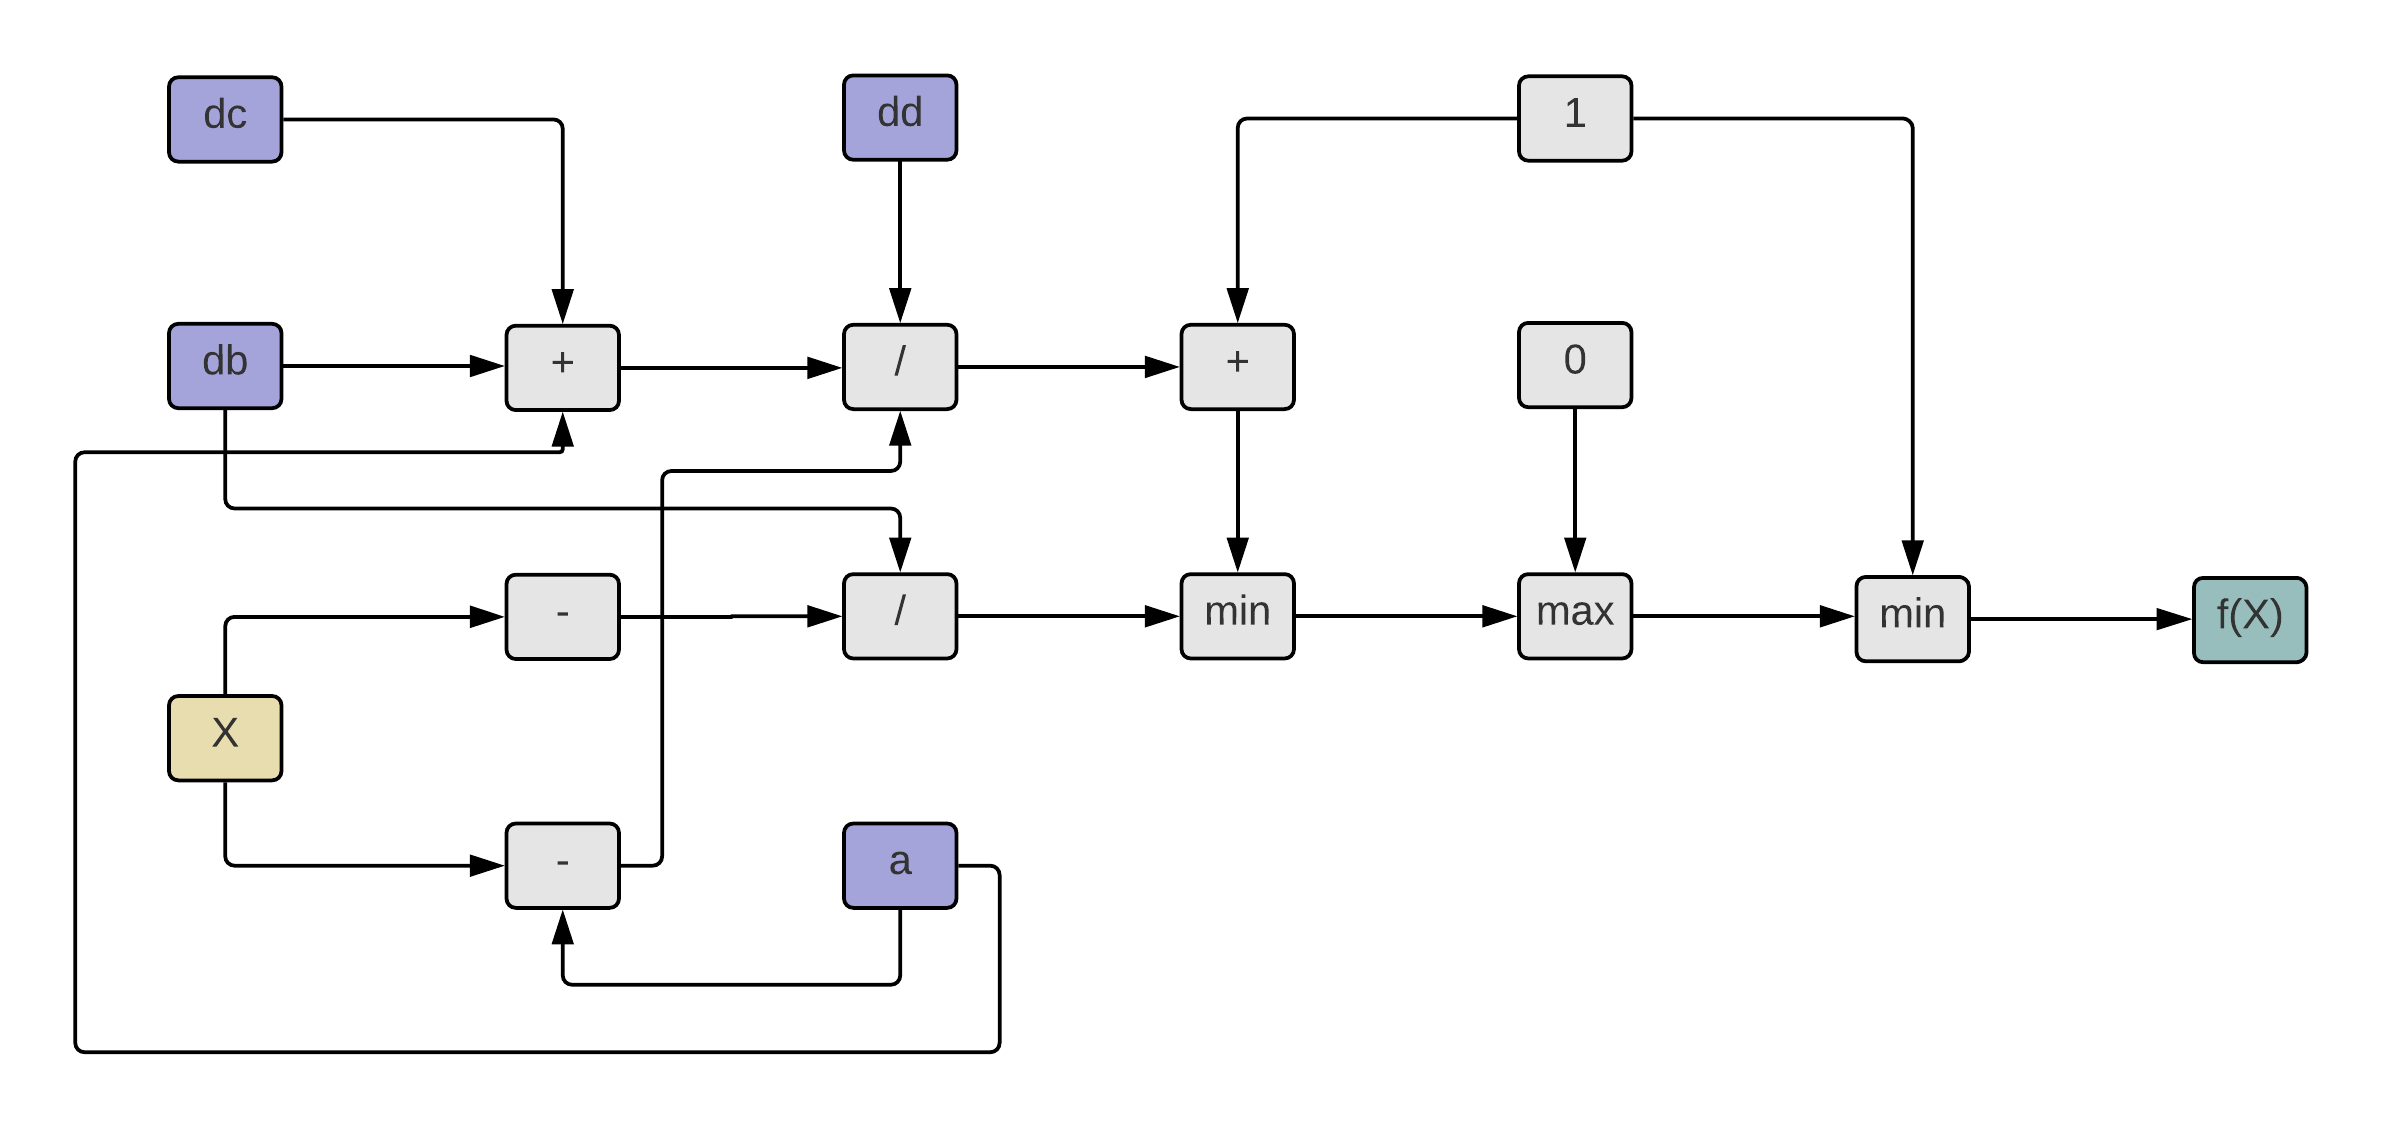
\includegraphics{trap-graph}
	\caption[Grafo computacional de la función de pertenencia para el trapecio]{Ilustración del grafo computacional para la función de pertenencia trapezoidal. La fórmula que describe es $\mu(x) = \min(\max(\min(\mu_{L_{asc}}, \mu_{L_{desc}}), 0), 1)$, esto es, una línea ascendente y otra descendente, estando ambas acotadas en el intervalo $[0, 1] \in \mathbb{R}$.}
	\label{fig:trap-grap}
\end{figure}

Sabiendo los grafos computacionales de cada una de las funciones de pertenencia, ya podemos definir el grafo asociado a la partición difusa de una variable lingüística. Suponiento que la variable $V$ está dividida en $n$ conjuntos difusos, la partición de ésta estará compuesta de:

\begin{itemize}
	\item Un primer conjunto definido como una pendiente descendente.
	\item $n - 2$ conjuntos definidos por una función de pertenencia de tipo trapezoidal.
	\item Un último conjunto definido como una pendiente ascendente.
\end{itemize}

Este grafo tiene que definir una serie de variables para que nuestro algoritmo de entrenamiento las ajuste correctamente. Estas variables están directamente relacionadas con los parámetros de las funciones de pertenencia descritas anteriormente. Hemos decidido por tanto establecer estas variables como los espacios existentes entre los puntos caracteríscos de las funciones. En la figura~\ref{fig:fuzzification-graph-vars} se puede observar de qué manera están relacionadas las variables de desplazamiento y los parámetros de las funciones de pertenencia.

\begin{figure}
	\centering
	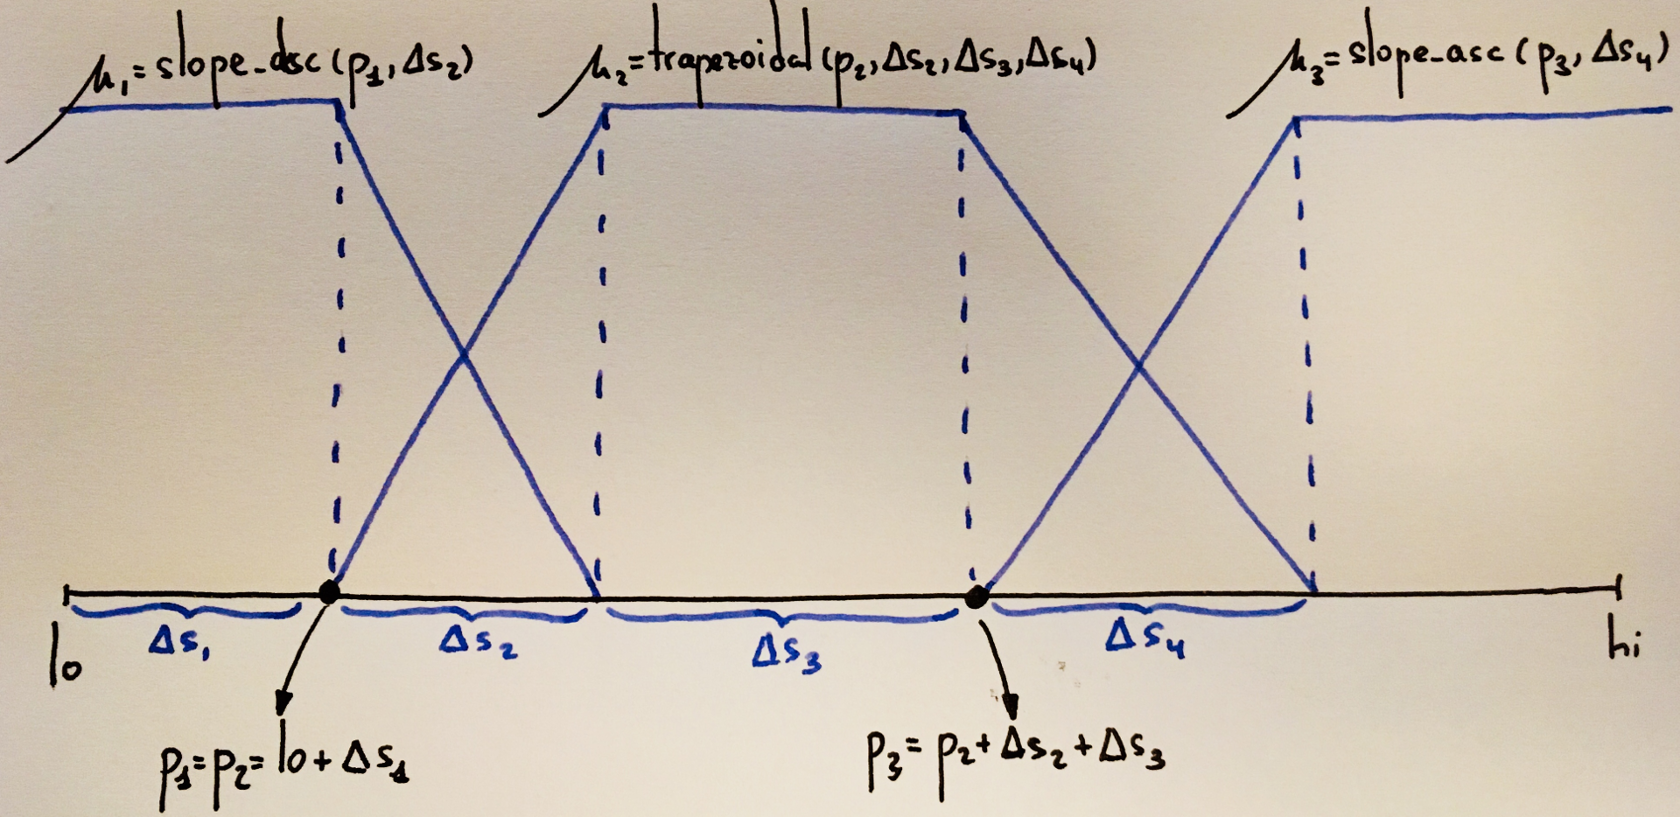
\includegraphics{fuzzification-graph-vars}
	\caption[Representación de una partición difusa para su ajuste]{Ilustración de una partición difusa para una variable lingüística con $n = 3$ conjuntos difusos en el dominio $[l, h]$. Al ser $n = 3$, la partición queda definida como un punto de origen $l$ y $2(n - 1)$ variables correspondientes a desplazamientos consecutivos, los cuales son los que definen los parámetros de las funciones de pertenencia de cada uno de los conjuntos difusos. A partir de este punto, los grafos computacionales son más complejos y su ilustración no aporta nada, por lo que los conceptos se ilustrarán de forma diferente.}
	\label{fig:fuzzification-graph-vars}
\end{figure}

Al estar definidas de esta manera, logramos (i) que la suma de todas las pertenencias en cada punto del eje $X$ es $1$ y (ii) que cada pequeña variación del gradiente de una de las variables tiene el potencial de provocar una variación en el resto de variables.

Por último, un controlador difuso define un número de variables de entrada. Nuestro grafo de fuzzificación estará definido de tal manera que para una matriz de entrada $m \times l$, siendo $m$ cada tupla de valores a inferir y $l$ cada una de las variables lingüísticas, generará una matriz de la forma $m \times \sum_{i=1}^l \left\vert{l_i}\right\vert$, siendo $\left\vert{S}\right\vert$ el número de conjuntos difusos que contiene la variable linguística $l_i$ (Figura~\ref{fuzzification-graph})

\begin{figure}
	\centering
	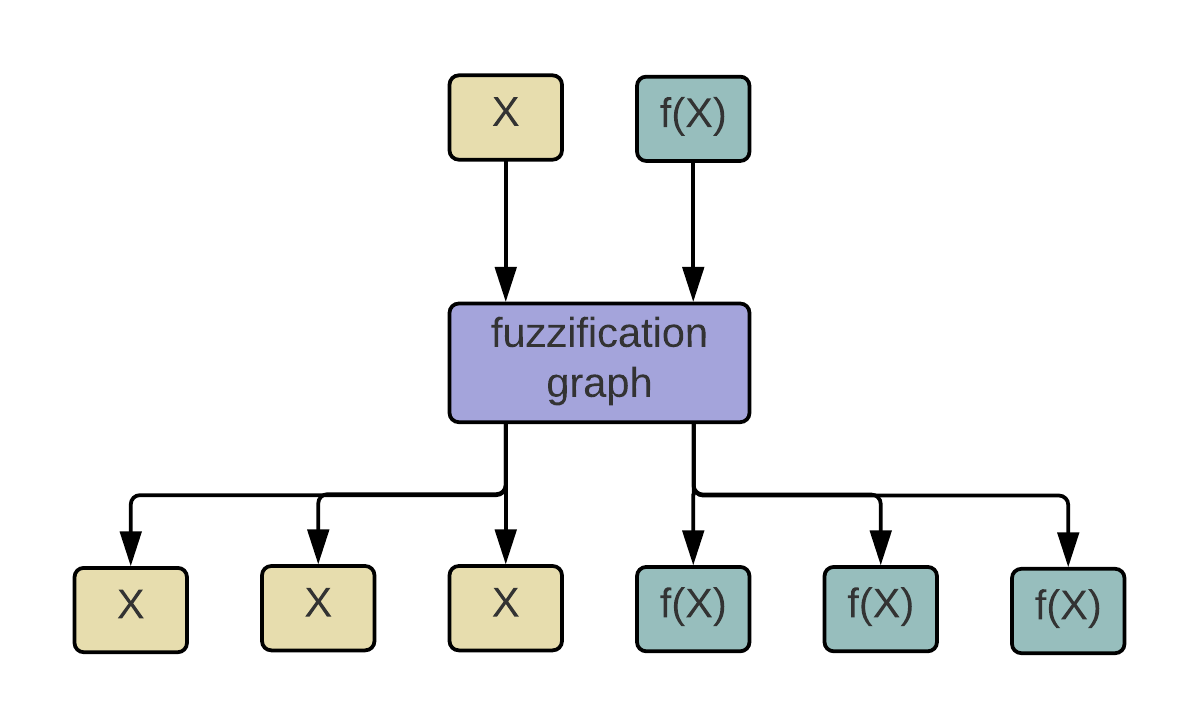
\includegraphics{fuzzification-graph}
	\caption[Ejemplo de operación de fuzzificación como grafo computacional]{Siendo el número de conjuntos difusos de las variables lingüísticas $X_1$ e $X_2$ $3$, el grafo de fuzzificación transformará los dos valores de entrada $x \in X_1$ e $y \in X_2$ en seis valores, los corerspondientes a los valores de pertenencia de $x$ e $y$ a cada uno de los conjuntos difusos de $X_1$ y $X_2$ respectivamente}
	\label{fig:fuzzification-graph}
\end{figure}

\newthought{La inferencia}, tomará esos valores difusos y generará los valores difusos de salida. Para ello, hará uso de un bloque de reglas en las que basará su inferencia.

Este bloque de reglas es el que se tratará de ajustar. La representación será la de una matriz $(v_i + 1)$-dimensional, siendo $v_i = \sum_{i=1}^l \left\vert{l_i}\right\vert$ (el número total de entradas difusas que llegan al bloque). La dimensión adicional se corresponde a la variable lingüística de salida.

Se puede pensar de esta manera. Para cada posible conjunto difuso de salida (es decir, para cada valor dentro del eje correspondiente a la salida), tenemos una matriz $v_i$-dimensional que se corresponde al producto cartesiano de las cariables de entradas. Esto es, cada una de las posibles combinaciones de reglas, a la que podemos asociar un valor. En la Figura~\ref{fig:inference-graph} se muestra un ejemplo con las variables obtenidas en el ejemplo de la Figura~\ref{fig:fuzzification-graph} tras aplicarles la $t$-norma.

\begin{figure}
	\centering
	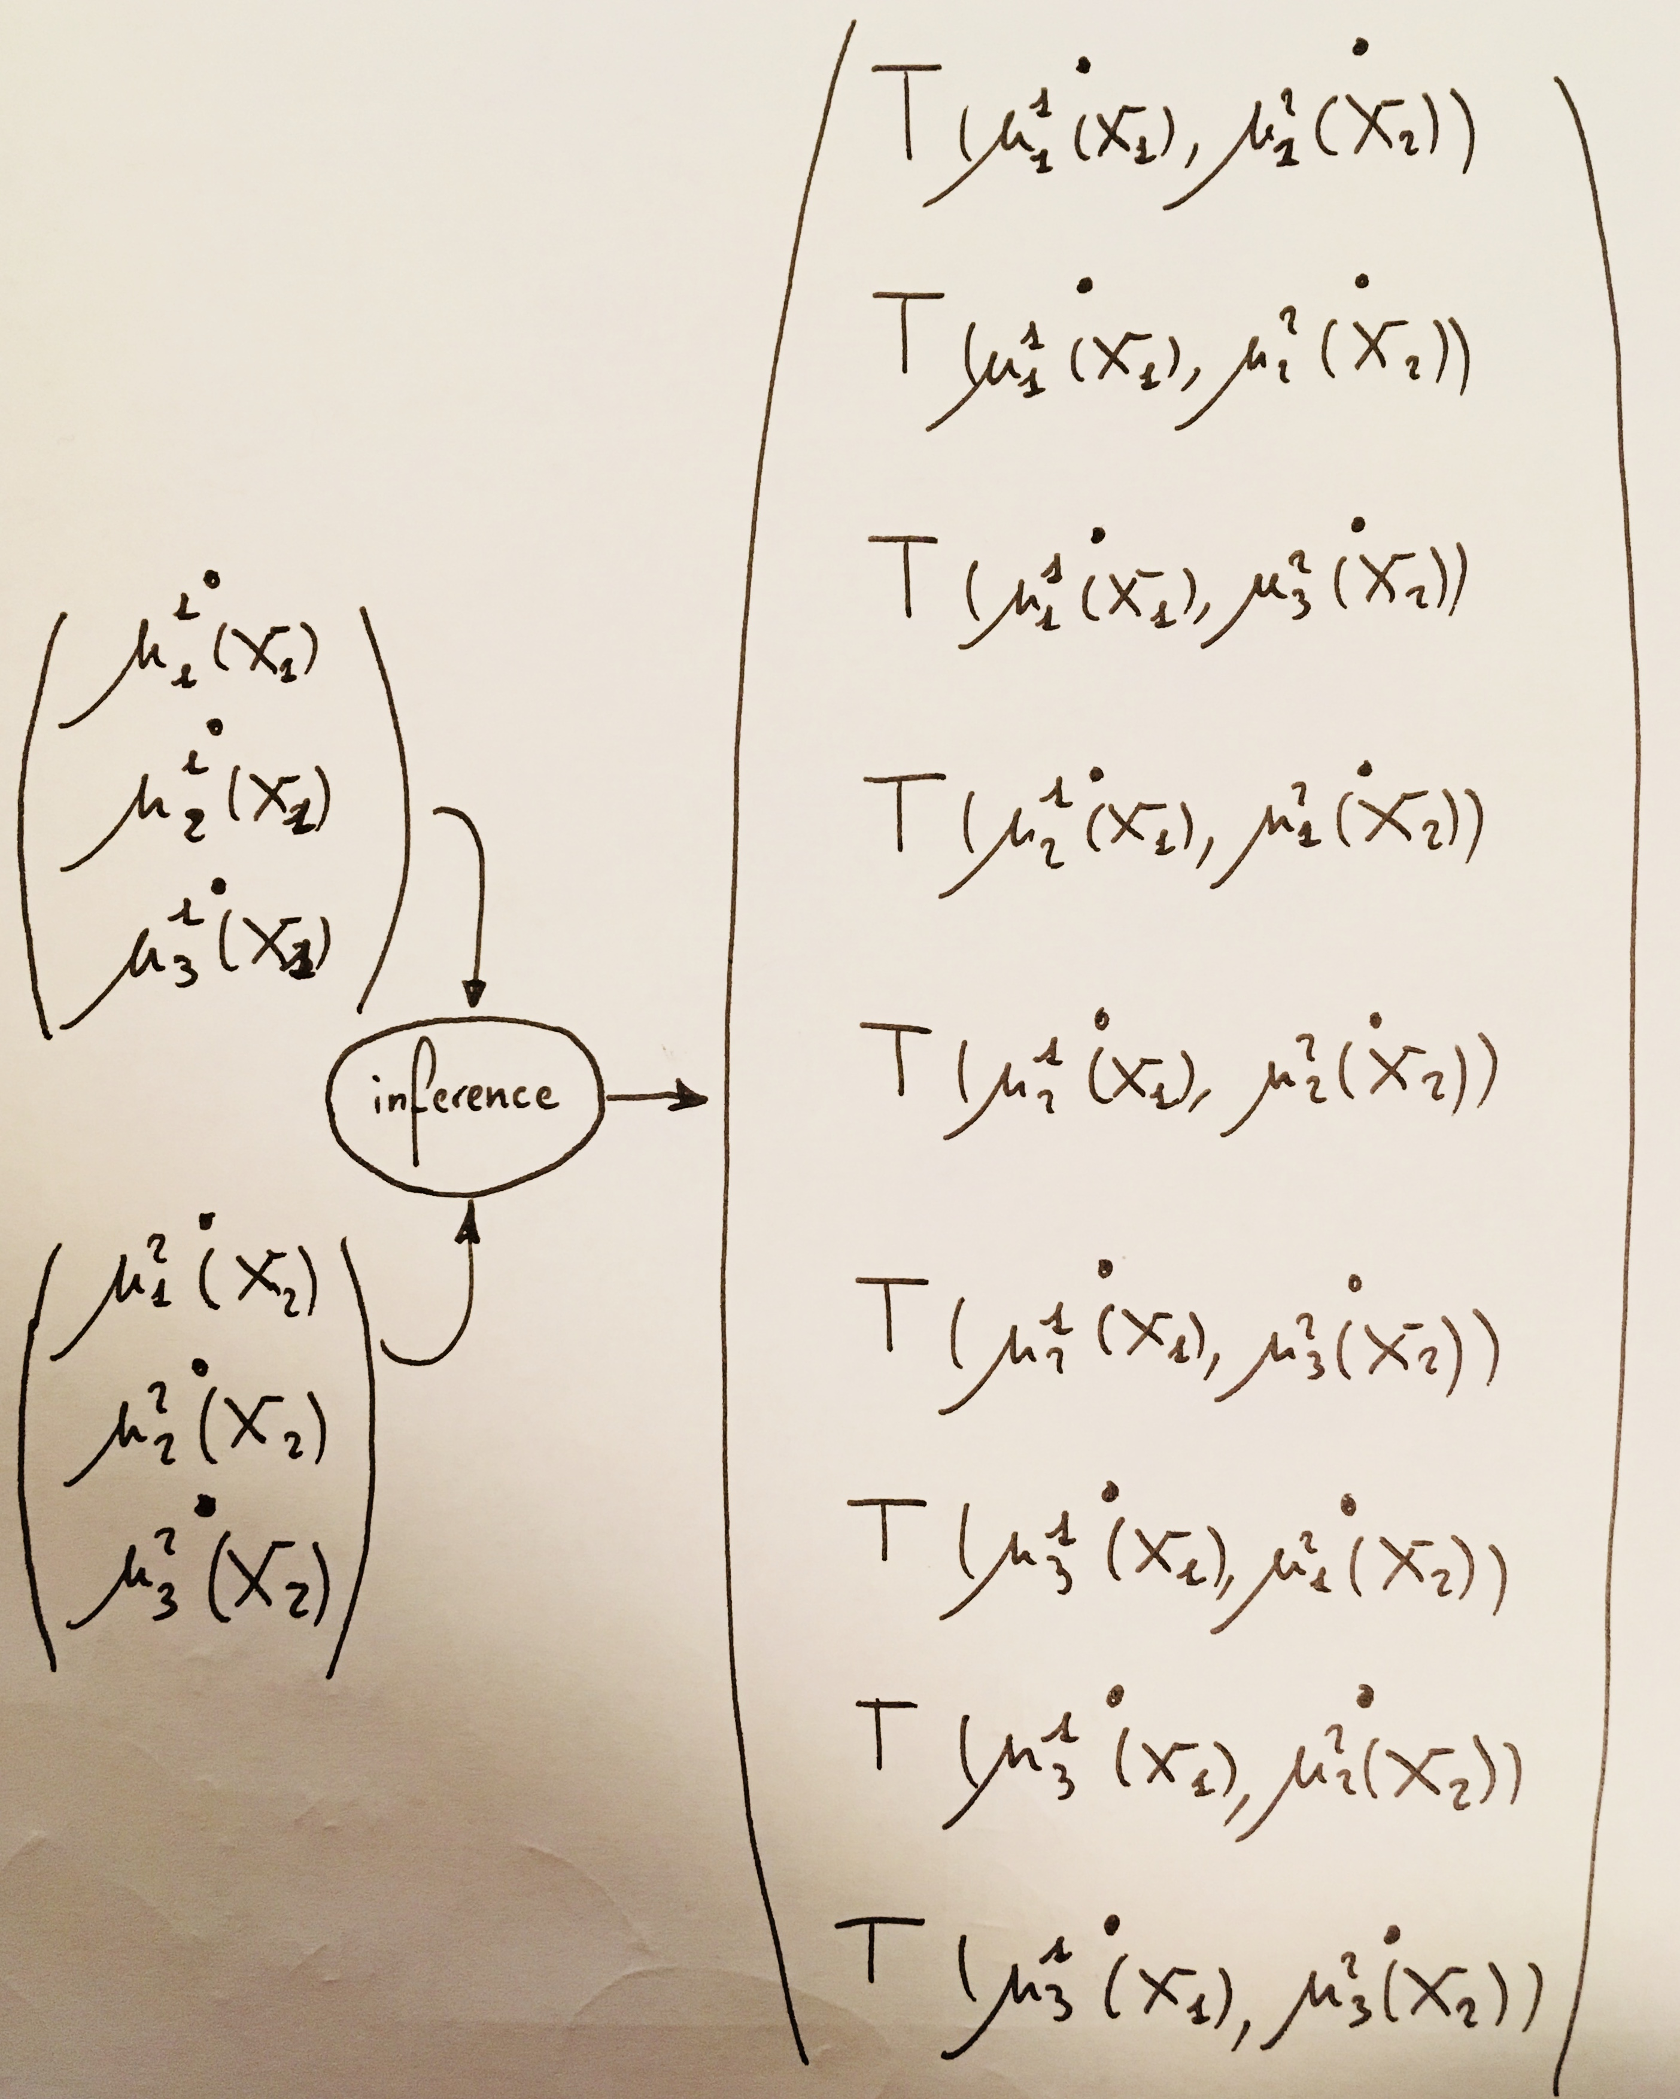
\includegraphics{inference-graph}
	\caption[Producto cartesiano de variables difusas de entrada]{El producto cartesiano de las variables difusas de entrada genera todas las posibles combinaciones entre los conjuntos difusos de las variables lingüísticas. Aplicándosele la $t$-norma a cada una de estas combinaciones tenemos todas las posibles reglas que se pueden definir en este \ac{fcs}.}
	\label{fig:inference-graph}
\end{figure}

Al estar definida la $t$-conorma y la acumulación con el mismo operador (i.e. el máximo), una regla de tipo OR es equivalente a dos reglas de tipo AND, ya que la acumulación de sus resultados es equivalente. Por tanto, al aplicar la $t$-norma a estas combinaciones tenemos todas las posibles combinaciones de reglas. Pero hasta aquí no tenemos ningún ajuste.

Si aplicamos el producto de hadamard contra una matriz de pesos con la misma dimensión y acotamos sus valores a $[0, 1] \in \mathbb{N}$, tenemos una manera de ajustar qué reglas son las más relevantes y cuáles no. Esta representación tiene un problema: las regiones definen meseta en la función de error, y por tanto en el momento que el gradiente cae en alguna de estas mesetas, la evolución de la variable se estanca. Sin embargo, si en lugar de un valor natural, el peso toma un valor real y le aplicamos una sigmoidal, el valor se mantendrá entre $(0, 1) \in \mathbb{R}$ con la ventaja de que el gradiente no se estanca, y en un proceso posterior se pueden descartar las reglas cuyos valores están próximos a $0$.

A la salida de la inferencia, tras aplicar la acumulación, disponemos de tantos valores difusos como conjuntos difusos tiene la salida.

\newthought{El último paso, la defuzzificación}, es una aplicación similar a las funciones de pertenencia, pero aquí no cabe lugar a ningún ajuste de variables.

De los valores difusos se obtiene un valor que será el correspondiente a la salida de nuestro \ac{fcs}.